\documentclass[11pt]{article}
\pagestyle{plain}
\usepackage{latexsym,exscale,amsfonts,amsmath,amssymb,array}
\usepackage{color}
\usepackage[colorlinks]{hyperref}
\setlength{\topmargin}{-2.3cm}
\setlength{\textheight}{23.8cm}
\setlength{\oddsidemargin}{-0.5cm}
\setlength{\textwidth}{17cm}
\setlength{\parindent}{0cm}
\setlength{\parskip}{.4cm}
\newcommand{\totaldiffx}{\frac{d}{dx}}
\newcommand{\pardiffx}{\frac{\partial}{\partial x}}
\newcommand{\luft}{\:\!}

\usepackage{graphicx}
\usepackage[latin1]{inputenc}
\usepackage{mathpazo}
\usepackage[T1]{fontenc}
\usepackage[comma,numbers,sort&compress]{natbib}


\begin{document}
\begin{center}
\large \bf Computational Astrophysics \rm \\
2019\\
{\small Exercises 12. Parabolic PDEs}
\end{center}

\textbf{Advection Equation} \\
Advection is an important process in many aspects of astrophysics. For example, some transport models consider shock-accelerated particle distributions in the heliosphere \cite{Litvinenko2014} that are described, in a first approximation, by a one-dimensional advection-difussion equation for the particle density. In the weak diffusion approximation the equation to solve is
\begin{equation}
\frac{\partial u}{\partial t} + v\frac{\partial u}{\partial x} = 0\,\,,
\end{equation}
where $v$ is a constant advection speed taht can be interpreted as the background solar wind speed \cite{Litvinenko2014}.
As a first example in solving partial differential equations, we will use this equation  to advect a Gaussian profile
\begin{equation}
 \Psi_0 = \Psi(x,t=0) = e^{-\frac{(x-x0)^2 }{(2 \sigma^2)}},
 \end{equation}
 with $x0 = 30$, $\sigma = \sqrt{15}$, with positive
velocity $v = 0.1$ in a $[0,100]$ domain.\\ 
In order to handle the boundaries, we will choose ``outflow'' boundary
conditions, that simply copy the data of the last interior grid point into the
boundary points.
\begin{center}
\vspace*{-0.4cm}
\begin{minipage}{0.4\textwidth}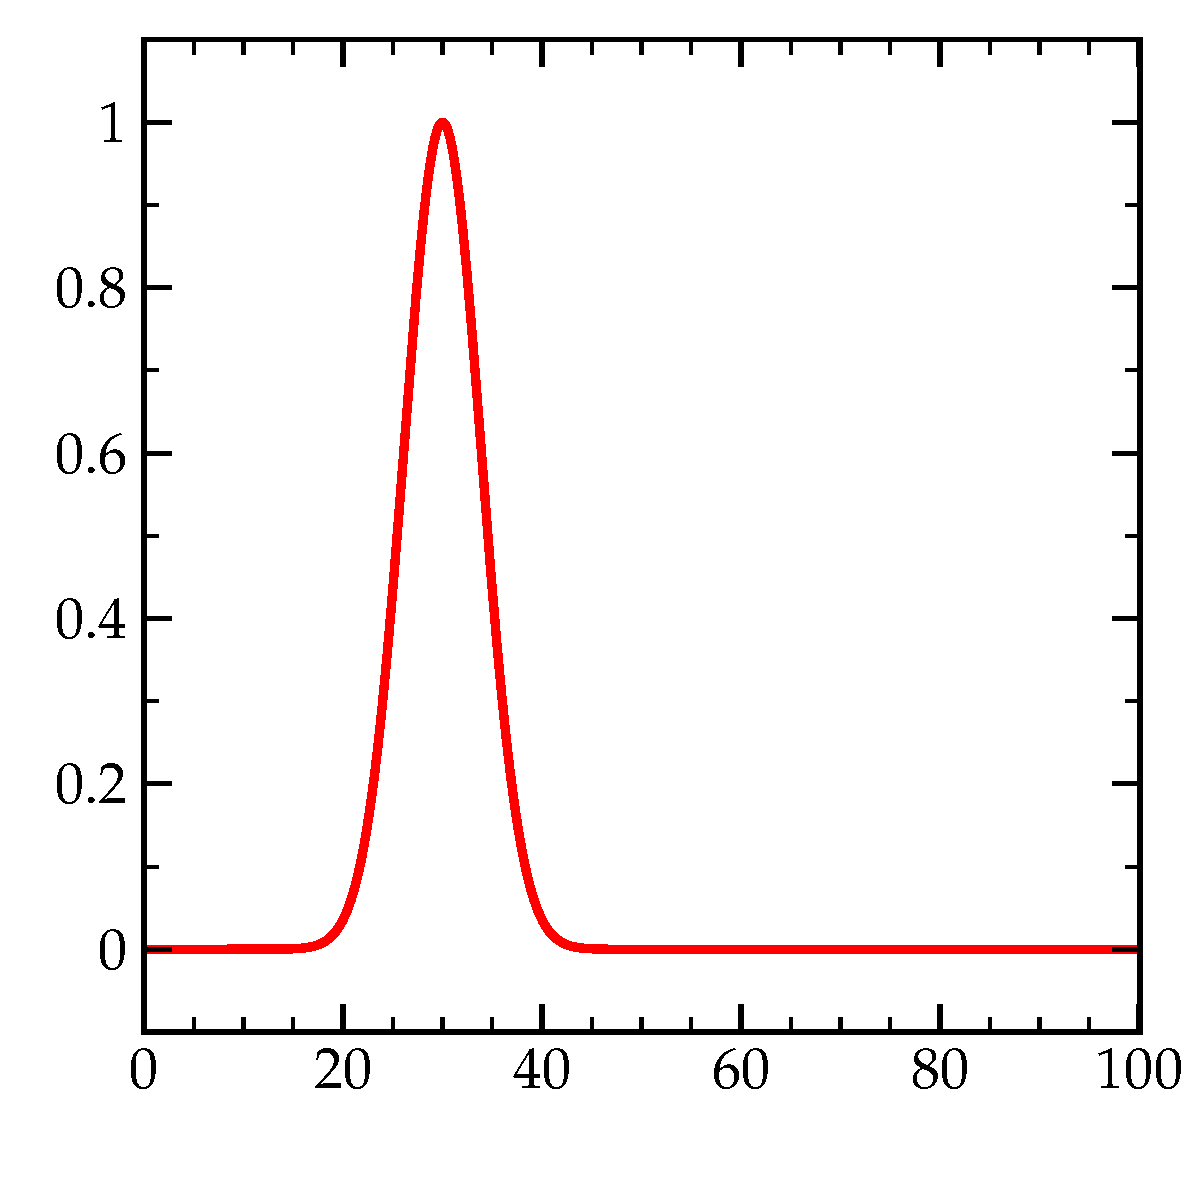
\includegraphics[width=1\textwidth]{gauss_advect_plot.pdf}
\end{minipage}
\vspace*{-0.5cm}
\end{center}
\renewcommand{\labelenumi}{(\arabic{enumi})}

\vspace*{-0.5cm}
\begin{enumerate}
\item[(2)] Implement the upwind scheme and demonstrate by experiment that
  it is stable for $0 \le \alpha = v \Delta t / \Delta x \le 1$. Implement
  an error measure and make a plot of the error as a function of time. Now
  try a Gaussian with a 5 times smaller $\sigma$. What do you observe regarding
  the error and the visual comparison with the analytic result?
  \vspace{0.1cm}


\item[(2)] Implement the unstable FTCS scheme and observe the development
  of instability. Make a few plots and describe what you observe.
  
  \item[(4)]Implement the Lax-Friedrich Method and
  compare it (visually) to upwinding. Make a few plots. Describe what
  you find.

\item[(5)] 
  Implement the Leapfrog scheme and Lax-Wendroff. Compare the two
  results.
  \end{enumerate}

Happy Coding :) !

\begin{thebibliography}{10}
\bibitem {Litvinenko2014} Y. E. Litvinenko and F. Effenberger. The Astrophysical Journal, \textbf{796}, 125 (2014)

\end{thebibliography}

\end{document}
